\section{Appendix}

%--------------------------------------------------------
%--------------------------------------------------------
\subsection{ Mathematical properties of spin spherical harmonics}\label{sec:ylm_mathprop}
The sum over $m$ index of product of two spherical harmonic functions of spin $s_1$ and $s_2$ respectively, is given by the following expression \cite{varshalovich},
\beq \label{eq:sum_spin_shf}
 \sum_{m}{_{s_1}Y^*_{\ell m}}(\hat{n}_i){_{s_2}Y_{\ell m}}(\hat{n}_j) = \sqrt{\frac{2\ell+1}{4 \pi}} _{s_2}Y^{-s_1}_{\ell}(\beta,\alpha) e^{- i s_2 \gamma} \,,
\eeq
where $\alpha, ~\beta ~\&~ \gamma$ correspond to the Euler angles that specify the rotation matrix which transforms the local cartesian coordinates defined at $\hat{n}_i$ such that it aligns with the local cartesian coordinate system at $\hat{n}_j$.

The spin spherical harmonics satisfy the following orthogonality relations,
%
\beq
\int  {_sY_{\ell m}}(\hat{n}){_sY^*_{\ell' m'}}(\hat{n}) d\Omega = \delta_{\ell \ell'} \delta_{\rm m m'} \,, \label{eq:ylmortho1}
\eeq
%
where $s$ denotes the spin of the spherical harmonic coefficients. The numerical validity of \eq{eq:ylmortho1} is only limited by the rate at which these functions are sampled on the sphere and hence this identity can be made arbitrarily accurate by choosing a sufficiently high sampling rate.
%While working with CMB polarization one is often dealing with spin-2 spherical harmonics. Here we derive some relation which we use while evaluating the real space projection operators,
%\beq
%\sum_{\ell m} {_2Y}_{\ell m}(\hat n_i) {_2Y}^*_{\ell m}(\hat n_j) = 
%\eeq

The spin spherical harmonic functions satisfy the following completeness relation,
%
\beq
\sum_{\ell m}{_sY_{\ell m}}(\hat{n}_i){_sY^*_{\ell m}}(\hat{n}_j) = \delta(\hat{n}_i - \hat{n}_j) \label{eq:ylmortho2} \,,
\eeq
%
Note that the numerical validity of \eq{eq:ylmortho2} is strictly true only when the sums over the indices $(\ell, m)$ run to infinity. This is never true in practice, since the measured data invariable are band limited owing to the finite resolution of the experiments. Hence this relation is only approximately true and in more realistic scenario takes up the following function form,
%
\beqry
\sum_{\ell=\ell_{\rm min}, m}^{\ell_{\rm max}}{_sY_{\ell m}}(\hat{n}_i){_sY^*_{\ell m}}(\hat{n}_j) &\approx& \delta(\hat{n}_i - \hat{n}_j) \label{eq:ylmortho2} \,, \\
&=& \sum_{\ell=\ell_{\rm min}}^{\ell_{\rm max}} \sqrt{\frac{2 \ell+1}{4 \pi}} {}_{s}Y^{-s}_{\ell}(\beta,\alpha) e^{-i s \gamma} \,, \nonumber
\eeqry
%
where $\alpha, \beta ~\&~ \gamma$ are the Euler angles relating the two directions $\hat{n}_i$ and $\hat{n}_j$. A specific case of this function with $(s=2, \ell_{\rm min}=2, \ell_{\rm max}=96)$ is depicted in the last two columns of \fig{fig:vis_kernel}.

%--------------------------------------------------------
%--------------------------------------------------------
\subsection{Asymptotic forms for the functions ${}_{\pm 2}f_{\ell}(\beta)$}\label{sec:asymptotic_f}
The functions ${}_{\pm}f_{\ell}(\beta)$ need to be evaluated close to $\beta= 0$ and $\beta=\pi$. Close to these values we cannot evaluate these functions using the relation given in  \eq{eq:rad_ker_quequbqu}, owing to the inverse $\sin(\beta)$ dependence of a number of terms. To overcome this issue, we use the asymptotic form of the Legendre polynomials as $\beta \rightarrow 0$,
%
\beq
P_{\ell}^2(\cos{\beta})=\sin^2(\beta) \frac{(\ell+2)!}{8(\ell-2)!} \,.
\eeq
%
Using the above limiting form, the functions ${}_{\pm}f_{\ell}(\beta)$ reduce to the following equations,
%
\beqry
\lim_{\beta \to 0}{}_{\pm}f_{\ell}(\beta)&=&\frac{1}{4} \sqrt{\frac{2 \ell+1}{4 \pi}} \Bigg\lbrace -\left[  (\ell-4) + \frac{1}{2} \ell(\ell-1)\sin^2(\beta) \pm 2 (\ell-1) \cos(\beta) \right] \nonumber \\ &+& \left[ (\ell-2) \cos(\beta) \pm 2(\ell-2) \right] \Bigg\rbrace \,.
\eeqry
%
Using the parity property of the associate Legendre polynomials: $P_{\ell}^m(-x)=(-1)^{\ell+m}P_{\ell}^{m}(x)$, the asymptotic form for the functions ${}_{\pm}f_{\ell}(\beta)$ in the limit $\beta \rightarrow \pi$ are given by the following equations,
%
\beqry
\lim_{\beta \to \pi}{}_{\pm}f_{\ell}(\beta)&=&\frac{1}{4} \sqrt{\frac{2 \ell+1}{4 \pi}} \Bigg\lbrace -\left[ (\ell-4) + \frac{1}{2} \ell(\ell-1)\sin^2(\beta) \pm 2 (\ell-1) \cos(\beta) \right] (-1)^{\ell} \nonumber \\ &+& \left[(\ell-2) \cos(\beta) \pm 2(\ell-2)\right] (-1)^{\ell-1} \Bigg\rbrace \,.
\eeqry
%
We use these asymptotic forms for ${}_{\pm}f_{\ell}(\beta)$ to evaluate the radial kernel close to the poles.
%--------------------------------------------------------
%--------------------------------------------------------
\subsection{Convolution error}\label{sec:convolution_err}
Here we assess  error in the simple integeration scheme used in our python script. To estimate the error, we use the Healpix integration scheme as the reference. The spatially local convolutions suggested in this work can be carried out using Healpix via the following algorithm: (i) Generate a disc mask of radius $r_{\rm cutoff}$ around a pixel with index ``i". (ii) Apply the mask on the Stokes Q \& U maps and evaluate the E \& B maps using standard Healpix functions. (iii) Store the E \& B field values evaluated at the pixel with index ``i" (the center of the disc mask), while rejecting the fields constructed at other pixels in the mask. (iv) Repeat this process at all pixels to generate a map of the scalar fields E \&  B.  This scheme is mathematical identical to our implementation of carrying out the convolution integrals over spatially local regions. In the above proposed algorithm the locality is enforced by the disc mask. However note that evaluating this scheme using Healpix is extremely inefficient since it effectively involves translating Npix Stokes Q \& U maps to scalar E \& B maps. The computational cost of carrying out this operation using Healpix grows quickly with the resolution parameter $\rm Nside$. For the results presented here we work with Healpix maps simulated at a resolution of Nside=64. 

We evaluate the E \& B maps using three different methods,  using our simple Python implementation of the local convolutions, the equivalent scheme using Healpix as described above and the full sky Healpix evaluation (which we use to evaluate the reference spectra). The relative percentage differences between the spectra derived from maps using the local methods and the reference spectra are depicted in \fig{fig:convolution-err}. Note that the error on the E mode spectrum derived from maps constructed using the two different local convolution methods nearly match each other. However for the B-mode spectrum, the error on the spectrum derived from our python implementation is significantly larger as compared to the error on the spectrum derived from the local Healpix convolution method. This indicated the fact that Healpix convolution has a better accuracy as compared our implementation. More important to note here is the fact that the error on the spectra from locally evaluated E and B mode maps are nearly equal to each other, as can be seen by comparing the green curves in the left and and right panels of \fig{fig:convolution-err}.
%
\begin{figure}[!h] 
\centering
\subfigure[]{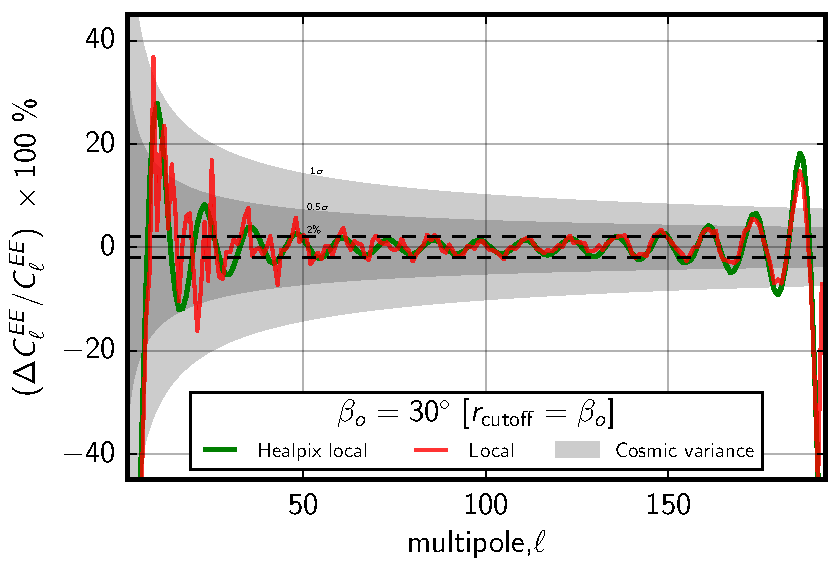
\includegraphics[width=0.49\columnwidth]{supplementary/convolution-err-ee-spectrum-radial-cutoff.pdf}}
\subfigure[]{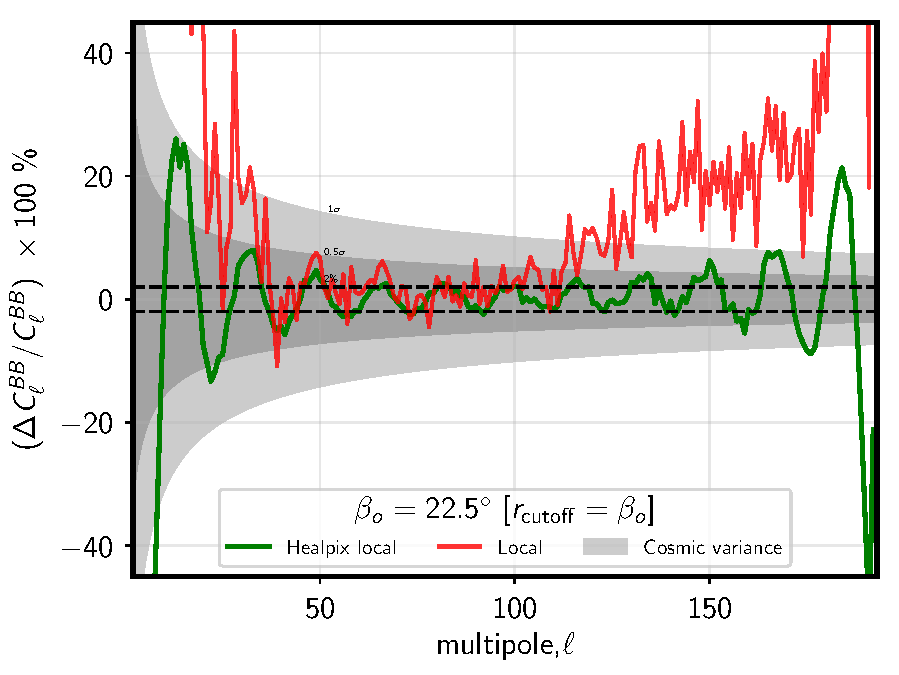
\includegraphics[width=0.49\columnwidth]{supplementary/convolution-err-bb-spectrum-radial-cutoff.pdf}}
\caption{The figure on the left and right depict the relative percentage difference between spectra derived from local convolution estimates of E \& B map and the reference spectra derived from full sky Healpix evaluations. The green curves depict the results from local E \& B maps evaluated using local Healpix operations while the red curve shows the same for the scalar maps derived using our python script. The gray band indicates the scatter expected due to cosmic variance, the lighter shade corresponding to $1\sigma$ and the darker shade to $0.5 \sigma$. \revisit{The cosmic variance band does not account for the non-guassian distribution, which is particularly relevant at the low multipoles.}}
\label{fig:convolution-err}
\end{figure}
%